\chapter{Cơ sở lý thuyết}
\section{Tổng quan về bệnh hại trên cây lúa}
\subsection{Bối cảnh và tầm quan trọng}
Cây lúa (\textit{Oryza sativa}) là cây lương thực chủ yếu của hơn 3.5 tỷ người trên thế giới, đặc biệt ở các nước châu Á. Trong vòng đời sinh trưởng, cây lúa dễ bị tấn công bởi nhiều loại mầm bệnh từ nấm, vi khuẩn và virus, gây thiệt hại kinh tế ước tính hàng chục tỷ USD mỗi năm. Tại Việt Nam, diện tích canh tác lúa đạt 7.1 triệu héc-ta với ba vụ thu hoạch mỗi năm; điều kiện khí hậu nhiệt đới ẩm tạo môi trường lý tưởng cho nhiều loại nấm và vi khuẩn phát triển, đặc biệt trong giai đoạn đẻ nhánh và làm đòng.

\subsection{Bệnh Đạo ôn (Rice Blast)}
\textbf{Tác nhân:} Nấm \textit{Pyricularia oryzae} (hay còn gọi là \textit{Magnaporthe oryzae}). Chu kỳ lây nhiễm bắt đầu từ bào tử nấm bám vào bề mặt lá và xâm nhập qua khí khổng hoặc trực tiếp qua lớp biểu bì.

\textbf{Triệu chứng đặc trưng:}
\begin{itemize}[leftmargin=1.5cm]
    \item Vết bệnh có hình thoi hoặc hình mắt chim, kích thước 1--2 cm.
    \item Tâm vết bệnh màu xám nhạt, viền màu nâu đậm hoặc vàng.
    \item Giai đoạn nặng: vết bệnh lan ra toàn bộ lá, lá héo khô.
    \item Bệnh tấn công cả cổ bông (cổ gié), gây lép hạt nghiêm trọng.
\end{itemize}

\textbf{Điều kiện phát triển:} Độ ẩm không khí cao ($>90\%$), nhiệt độ $20$--$28^\circ$C, trời âm u có sương mù là môi trường thuận lợi nhất. Bón thừa đạm là nguyên nhân chính kích thích bệnh bùng phát.

\subsection{Bệnh Bạc lá (Bacterial Leaf Blight)}
\textbf{Tác nhân:} Vi khuẩn \textit{Xanthomonas oryzae pv. oryzae} --- một trong những tác nhân gây bệnh cây trồng nguy hiểm nhất thế giới. Vi khuẩn xâm nhập qua vết thương cơ học hoặc khí khổng, nhân lên nhanh chóng trong mô lá và tiết ra enzyme phá vỡ thành tế bào.

\textbf{Triệu chứng đặc trưng:}
\begin{itemize}[leftmargin=1.5cm]
    \item Dải vàng hoặc trắng bạc chạy dọc theo mép lá, từ chóp lá lan xuống.
    \item Ranh giới giữa vùng bệnh và vùng khỏe không rõ ràng, có dạng lượn sóng.
    \item Buổi sáng sớm có thể quan sát thấy giọt dịch vi khuẩn màu đục vàng nhạt đọng ở mép lá --- đây là dấu hiệu đặc trưng nhất để phân biệt bạc lá với các bệnh khác.
    \item Lá bệnh khô và cuộn lại từ mép vào trong.
\end{itemize}

\textbf{Điều kiện phát triển:} Nhiệt độ $28$--$32^\circ$C, độ ẩm cao, mưa to gió lớn là điều kiện lây lan mạnh nhất. Bệnh đặc biệt nghiêm trọng trong vụ hè thu tại Đồng bằng sông Cửu Long.

\subsection{Bệnh Đốm nâu (Brown Spot)}
\textbf{Tác nhân:} Nấm \textit{Bipolaris oryzae} (đồng danh \textit{Helminthosporium oryzae}). Đây là bệnh có lịch sử lâu đời nhất và liên quan đến nạn đói Bengal năm 1943, nơi bệnh đốm nâu phá hủy phần lớn mùa màng lúa ở Ấn Độ.

\textbf{Triệu chứng đặc trưng:}
\begin{itemize}[leftmargin=1.5cm]
    \item Vết bệnh hình tròn hoặc bầu dục, màu nâu đậm, kích thước bằng hạt vừng đến hạt đậu.
    \item Tâm vết bệnh có thể chuyển màu xám nhạt ở giai đoạn muộn, bao quanh bởi quầng vàng nhạt.
    \item Phân bố tản mạn, không theo hướng gân lá như bệnh bạc lá.
\end{itemize}

\textbf{Điều kiện phát triển:} Ruộng nghèo dinh dưỡng (thiếu Kali, Silic), đất phèn, ngộ độc hữu cơ. Nhiệt độ $16$--$36^\circ$C, độ ẩm $86$--$100\%$.

\subsection{Bệnh Vàng lùn --- Tungro}
\textbf{Tác nhân:} Phức hợp hai loại virus: \textit{Rice tungro spherical virus} (RTSV) và \textit{Rice tungro bacilliform virus} (RTBV). Đặc biệt, bệnh không lây trực tiếp từ cây sang cây mà phụ thuộc hoàn toàn vào vật trung gian là rầy xanh đuôi đen (\textit{Nephotettix virescens}).

\textbf{Triệu chứng đặc trưng:}
\begin{itemize}[leftmargin=1.5cm]
    \item Cây lúa bị lùn lại rõ rệt so với cây khỏe mạnh cùng lứa tuổi.
    \item Lá có màu vàng cam hoặc vàng nhạt, bắt đầu từ chóp lá lan dần xuống gốc.
    \item Khác với triệu chứng thiếu đạm, màu vàng do Tungro thường không đồng đều, lốm đốm.
    \item Số bông giảm, hạt lép nhiều, năng suất có thể giảm đến 100\%.
\end{itemize}

\textbf{Điều kiện phát triển:} Mật độ rầy xanh đuôi đen cao, đặc biệt trong điều kiện thời tiết nóng ẩm, nhiệt độ $25$--$30^\circ$C và độ ẩm không khí trên $80\%$. Ruộng gieo sạ dày, bón thừa đạm, canh tác liên tục nhiều vụ và còn lúa chét là điều kiện thuận lợi cho rầy phát sinh, lan truyền virus nhanh chóng.

\begin{table}[H]{So sánh đặc điểm nhận dạng bốn loại bệnh lúa phổ biến}
\centering
\small
\setlength{\tabcolsep}{4pt}
\begin{tabular}{>{\bfseries}p{2.6cm} p{3.2cm} p{3.2cm} p{3.2cm} p{3.2cm}}
\toprule
\textbf{Đặc điểm} & \textbf{Đạo ôn} & \textbf{Bạc lá} & \textbf{Đốm nâu} & \textbf{Vàng lùn} \\
\midrule
Tác nhân & Nấm \textit{P. oryzae} & Vi khuẩn \textit{X. oryzae} & Nấm \textit{B. oryzae} & \textit{RTSV, RTBV}\\[4pt]
Đặc điểm nhận dạng & Vết bệnh màu xám, viền nâu vàng, có hình thoi, mắt chim & Dải bệnh màu vàng, trắng & Vết bệnh màu nâu, có hình tròn, bầu dục & Cây lùn, vàng lá\\[4pt]
Phân bố & Rải rác trên lá & Dọc theo mép lá & Tản mạn toàn lá \\[4pt]
Điều kiện & Ẩm, mát, có sương & Nóng, ẩm, gió lớn & Đất nghèo dinh dưỡng & Mật độ rầy xanh cao, thời tiết nóng ẩm\\[4pt]
Nguy hiểm & Rất cao & Cao & Trung bình--cao & Cao\\
\bottomrule
\end{tabular}
\end{table}

\section{Tổng quan tình hình nghiên cứu}

\subsection{Các nghiên cứu sử dụng CNN trong phát hiện bệnh cây trồng}

Từ khoảng năm 2016, các mạng tích chập sâu (CNN) bắt đầu được áp dụng rộng rãi vào bài toán nhận dạng bệnh cây trồng qua ảnh. Mohanty et al. (2016) \cite{mohanty2016} là một trong những nghiên cứu tiên phong, sử dụng mạng AlexNet và GoogLeNet để phân loại 26 loại bệnh trên 14 loại cây, đạt độ chính xác 99.35\% trên tập kiểm thử từ bộ dữ liệu PlantVillage. Tuy nhiên, bộ dữ liệu này được chụp trong điều kiện phòng thí nghiệm --- nền đồng nhất, ánh sáng kiểm soát --- nên khi áp dụng vào điều kiện thực địa, hiệu năng sụt giảm đáng kể do nền phức tạp, ánh sáng thay đổi và góc chụp không nhất quán.

Riêng với cây lúa, Sethy et al. (2020) \cite{sethy2020} đề xuất phương pháp kết hợp CNN để trích xuất đặc trưng và SVM để phân loại, đạt 98.33\% trên tập dữ liệu lá lúa. Jiang et al. (2019) \cite{jiang2019} thử nghiệm ResNet-50 trên ảnh bệnh lúa thu thập tại Trung Quốc và nhận xét rằng khả năng mô hình hóa các phụ thuộc tầm xa là hạn chế lớn nhất của CNN khi xử lý các vết bệnh phân bố không đồng đều trên lá. Đây cũng là động lực chính để tác giả chuyển sang kiến trúc Vision Transformer trong đề tài này.

Điểm chung của các nghiên cứu CNN là: hiệu năng cao trên tập kiểm thử nhưng dễ suy giảm khi gặp ảnh thực địa, khó giải thích quyết định phân loại, và thường chỉ dừng ở bước phân loại mà không tích hợp thêm tri thức bệnh học hay khuyến nghị điều trị.
\newpage
\subsection{Ứng dụng Vision Transformer trong nhận dạng bệnh cây trồng}

Sau khi Dosovitskiy et al. (2021) \cite{dosovitskiy2020} chứng minh ViT có thể cạnh tranh với CNN trên ImageNet khi có đủ dữ liệu tiền huấn luyện, nhiều nhóm nghiên cứu đã thử nghiệm ViT cho bài toán bệnh cây trồng. Chen et al. (2021) \cite{chen2021} so sánh ViT-Base với ResNet-50 trên tập dữ liệu PlantVillage và cho thấy ViT vượt trội 2--3\% F1-score, đặc biệt trên các lớp bệnh có hình thái phức tạp như đốm vòng và thối nhũn.

Saleem et al. (2022) \cite{saleem2022} ứng dụng ViT kết hợp với Grad-CAM để trực quan hóa vùng lá mà mô hình chú ý nhiều nhất, giúp tăng tính giải thích. Nghiên cứu này chỉ ra rằng ViT có xu hướng tập trung vào biên của vết bệnh --- nơi ranh giới giữa mô khỏe và mô bệnh rõ ràng nhất --- trong khi CNN thường kích hoạt trên vùng trung tâm vết bệnh.

Đối với lúa cụ thể, Islam et al. (2022) \cite{islam2022} fine-tune ViT-Base trên bộ dữ liệu gồm 5 loại bệnh lúa thu thập tại Bangladesh, đạt F1 = 0.961 --- gần với kết quả của đề tài này (F1 = 0.963). Điểm khác biệt là nghiên cứu đó dừng lại ở bước phân loại; đề tài này bổ sung thêm phân tích hình thái học và cơ chế RAG để cung cấp thông tin điều trị.

\subsection{Ứng dụng LLM và RAG trong nông nghiệp thông minh}

Việc tích hợp mô hình ngôn ngữ lớn vào các hệ thống nông nghiệp còn khá mới. Khichar et al. (2023) \cite{khichar2023} trình bày chatbot nông nghiệp dựa trên GPT-3.5, cho phép nông dân đặt câu hỏi về sâu bệnh và nhận câu trả lời bằng ngôn ngữ tự nhiên. Tuy nhiên, hệ thống không có cơ chế RAG nên hay bị hallucination --- đặc biệt với các khuyến nghị liều lượng thuốc trừ sâu.

RAG (Retrieval-Augmented Generation) được Lewis et al. (2020) \cite{lewis2020} đề xuất như một giải pháp kết hợp ưu điểm của hệ thống truy xuất thông tin truyền thống và khả năng sinh ngôn ngữ của LLM. Ứng dụng RAG trong nông nghiệp còn hạn chế, nhưng Mohanty et al. (2023) \cite{mohanty2023} đã thử nghiệm với ChromaDB và cho thấy RAG giảm tỷ lệ hallucination từ 23\% xuống còn 4\% so với LLM thuần túy khi trả lời câu hỏi về bệnh cây trồng.

Điểm mà đề tài này đóng góp so với các nghiên cứu trên là kết hợp \emph{đồng thời} ba thành phần: ViT cho phân loại, Gemini Vision cho phân tích hình thái đa phương thức, và RAG với ChromaDB cho tri thức bệnh học --- tất cả được tổ chức dưới kiến trúc đa tác nhân để dễ bảo trì và mở rộng.

\newpage
\section{Mạng nơ-ron tích chập CNN và giới hạn}

\subsection{Lịch sử phát triển CNN}
Mạng nơ-ron tích chập (Convolutional Neural Network — CNN) được giới thiệu lần đầu bởi LeCun et al. vào năm 1989, dựa trên ý tưởng mô phỏng cơ chế xử lý thị giác của não người, trong đó các tế bào thần kinh chỉ phản ứng với một vùng cục bộ của trường thị giác. Kiến trúc này sử dụng các lớp tích chập (convolutional layers) để tự động học các đặc trưng không gian từ ảnh thông qua các bộ lọc (filters/kernels), thay vì phải thiết kế đặc trưng thủ công như các phương pháp truyền thống. Ý tưởng này được hiện thực hóa đầy đủ và trở nên nổi tiếng với kiến trúc LeNet-5 (1998) — một mạng gồm các lớp tích chập, pooling và fully connected, được áp dụng thành công vào bài toán nhận dạng chữ số viết tay trên tập dữ liệu MNIST.
\\\indent Tuy nhiên, do hạn chế về dữ liệu và sức mạnh tính toán, CNN chưa thực sự bùng nổ cho đến cột mốc bước ngoặt năm 2012, khi AlexNet của Krizhevsky et al. giành chiến thắng cuộc thi phân loại ảnh ImageNet Large Scale Visual Recognition Challenge (ILSVRC) với tỷ lệ lỗi top-5 chỉ khoảng 15,3\% — thấp hơn gần 10 điểm phần trăm so với đội xếp thứ hai sử dụng các phương pháp truyền thống. AlexNet có kiến trúc sâu hơn LeNet đáng kể với 5 lớp tích chập và 3 lớp fully connected, đồng thời tận dụng GPU để tăng tốc huấn luyện và áp dụng các kỹ thuật như hàm kích hoạt ReLU, dropout để chống overfitting. Chiến thắng này đã mở ra kỷ nguyên học sâu trong thị giác máy tính, thuyết phục cộng đồng nghiên cứu rằng deep learning là con đường đúng đắn.
\\\indent Tiếp nối thành công đó, hàng loạt kiến trúc CNN mới ra đời và liên tiếp phá kỷ lục độ chính xác trên ImageNet. VGGNet (2014) của nhóm Visual Geometry Group — Oxford chứng minh rằng độ sâu của mạng là yếu tố then chốt, bằng cách xếp chồng nhiều lớp tích chập 3×3 nhỏ thay vì dùng các bộ lọc lớn, đạt độ chính xác vượt trội với kiến trúc 16–19 lớp đơn giản và đồng nhất. Cùng năm đó, GoogLeNet/Inception (2014) của Google đề xuất mô-đun Inception — cho phép thực hiện tích chập với nhiều kích thước bộ lọc song song rồi ghép kết quả lại — giúp mạng vừa sâu vừa rộng mà không làm tăng quá mức chi phí tính toán. Đến năm 2015, ResNet (Residual Network) của He et al. tại Microsoft Research giải quyết triệt để vấn đề vanishing gradient trong mạng rất sâu bằng cơ chế kết nối tắt (skip connection / residual connection), cho phép huấn luyện các mạng lên đến 152 lớp và đạt tỷ lệ lỗi top-5 chỉ 3,57\% trên ImageNet — thậm chí vượt qua độ chính xác của con người trong bài toán này.
\newpage
\subsection{Cơ chế hoạt động của CNN}
\textbf{Tích chập (Convolution):} Lõi của CNN là phép toán tích chập --- áp dụng một bộ lọc (filter/kernel) kích thước $k \times k$ lên vùng cục bộ của ảnh đầu vào:
\begin{equation}
    (I * K)(i,j) = \sum_{m=0}^{k-1} \sum_{n=0}^{k-1} I(i+m,\, j+n) \cdot K(m,n)
    \label{eq:convolution}
\end{equation}
trong đó $I$ là ảnh đầu vào, $K$ là bộ lọc và $(i,j)$ là tọa độ pixel đầu ra.

\textbf{Pooling:} Sau mỗi lớp tích chập, max-pooling giảm kích thước không gian bằng cách lấy giá trị lớn nhất trong vùng $2\times2$, giúp mô hình bất biến với dịch chuyển nhỏ và giảm tham số.

\textbf{ReLU:} Hàm kích hoạt phi tuyến $f(x) = \max(0, x)$ được áp dụng sau mỗi lớp tích chập để tăng khả năng học biểu diễn phi tuyến.

\begin{figure}[H]{Kiến trúc điển hình của mạng CNN: ảnh đầu vào qua nhiều lớp Conv+Pool, sau đó Flatten và các lớp Fully Connected để phân loại.}
    \centering
    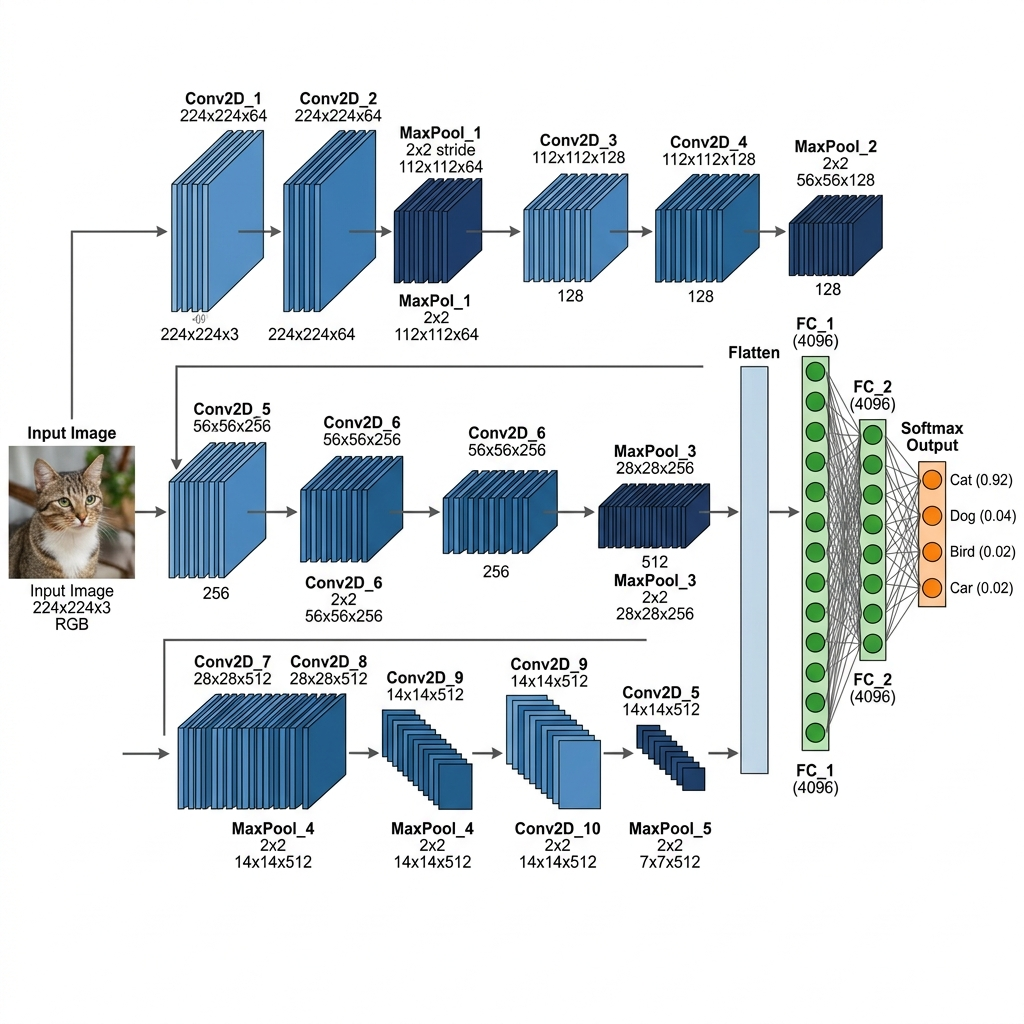
\includegraphics[width=0.9\textwidth]{docs/images/cnn_architecture.png}
\end{figure}

\subsection{Giới hạn của CNN trong nhận dạng bệnh lúa}
Mặc dù CNN đã chứng minh hiệu quả cao trong nhiều bài toán thị giác máy tính, song kiến trúc này mang những hạn chế cố hữu xuất phát từ chính thiết kế nền tảng của nó, đặc biệt bộc lộ rõ khi áp dụng vào bài toán phân tích hình thái bệnh lúa — một lĩnh vực đòi hỏi sự hiểu biết không gian tinh tế và khả năng diễn giải kết quả minh bạch.

\begin{enumerate}[leftmargin=1.5cm]
    \item \textbf{Trường thụ cảm cục bộ (Local Receptive Field):} Mỗi nơ-ron tích chập trong CNN chỉ xử lý một vùng không gian nhỏ của ảnh đầu vào, được giới hạn bởi kích thước bộ lọc (thường là 3×3 hoặc 5×5 pixel). Điều này có nghĩa là mô hình về bản chất chỉ "nhìn thấy" thông tin cục bộ tại mỗi bước xử lý. Để học được các phụ thuộc tầm xa (long-range dependencies) — ví dụ như mối liên hệ giữa vết bệnh xuất hiện ở đầu lá và các đốm hoại tử ở gốc lá — CNN buộc phải tích lũy thông tin qua rất nhiều lớp tích chập liên tiếp. Quá trình này không chỉ tốn kém về mặt tính toán mà còn kém hiệu quả, do thông tin toàn cục dễ bị suy giảm hoặc biến dạng khi truyền qua nhiều lớp biến đổi phi tuyến. Trong bài toán nhận dạng bệnh lúa, việc nắm bắt các mẫu phân bố không gian rộng — như sự lan rộng của đốm vân nâu hay hướng phát triển của vết cháy lá — là yếu tố quan trọng mà CNN xử lý chưa thực sự thỏa đáng.
    \item \textbf{Bất biến dịch chuyển:} CNN được thiết kế có chủ đích để đạt tính bất biến với phép dịch chuyển (translation invariance), tức là mô hình nhận dạng một đối tượng như nhau dù nó xuất hiện ở bất kỳ vị trí nào trong ảnh. Đây là ưu điểm trong nhiều bài toán phân loại ảnh tổng quát, nhưng lại trở thành hạn chế đáng kể trong phân tích bệnh lúa. Trên thực tế, vị trí tuyệt đối của vết bệnh trên lá mang thông tin chẩn đoán quan trọng: bệnh đạo ôn (blast) thường xuất hiện ở chóp lá hoặc cổ bông, bệnh khô vằn (sheath blight) tập trung ở bẹ lá phía dưới gần mặt nước, trong khi bệnh bạc lá (bacterial leaf blight) thường khởi phát từ mép lá. Khi CNN xóa bỏ thông tin vị trí thông qua các lớp pooling, những tín hiệu không gian có giá trị này bị mất đi, làm giảm khả năng phân biệt chính xác giữa các loại bệnh có hình thái vết bệnh tương đồng.
    \item \textbf{Phụ thuộc vào quy mô:} Kích thước vết bệnh trên lúa có thể dao động rất lớn tùy theo giai đoạn phát triển của bệnh, điều kiện môi trường và giống lúa — từ những đốm nhỏ vài milimet ở giai đoạn khởi phát đến các vùng hoại tử rộng hàng centimet ở giai đoạn bệnh nặng. CNN với các bộ lọc có kích thước cố định gặp khó khăn đáng kể khi cần nhận dạng cùng một loại bệnh ở các tỷ lệ khác nhau. Để khắc phục, người ta phải tích hợp các kỹ thuật bổ sung như multi-scale feature extraction hay Feature Pyramid Network (FPN) — tức là xây dựng các nhánh xử lý song song ở nhiều độ phân giải khác nhau rồi hợp nhất thông tin lại. Điều này làm tăng đáng kể độ phức tạp của kiến trúc, chi phí huấn luyện, cũng như khó khăn trong việc tinh chỉnh siêu tham số, trong khi hiệu quả đạt được vẫn chưa thực sự nhất quán trên mọi điều kiện thu thập ảnh thực địa.
    \item \textbf{Giải thích kém:} CNN về bản chất là một "hộp đen" (black box): mặc dù mô hình có thể đưa ra dự đoán với độ chính xác cao, nhưng quá trình ra quyết định bên trong — tại sao mô hình phân loại một mẫu bệnh cụ thể là đạo ôn thay vì đốm nâu — gần như không thể diễn giải một cách trực tiếp. Các kỹ thuật trực quan hóa như Grad-CAM hay saliency maps chỉ cung cấp được những gợi ý mờ nhạt về vùng ảnh mà mô hình "chú ý" đến, chứ chưa giải thích được cơ chế ra quyết định một cách thực sự tường minh. Đây là hạn chế đặc biệt nghiêm trọng trong các ứng dụng nông nghiệp và y tế thực tiễn, nơi người dùng cuối — như các kỹ sư nông nghiệp, nhà nghiên cứu bệnh cây, hay nông dân — cần hiểu được căn cứ của dự đoán để quyết định biện pháp xử lý phù hợp, đồng thời đặt ra yêu cầu về trách nhiệm giải trình (accountability) đối với hệ thống hỗ trợ quyết định.
\end{enumerate}

\section{Vision Transformer (ViT)}

\subsection{Từ xử lý ngôn ngữ tự nhiên (NLP) sang Thị giác máy tính}

Tiến trình phát triển của kiến trúc Transformer bắt đầu từ cột mốc quan trọng vào năm 2017, khi Vaswani cùng các cộng sự chính thức giới thiệu mô hình này nhằm giải quyết triệt để bài toán dịch máy trong lĩnh vực NLP. Khác biệt hoàn toàn với các kiến trúc truyền thống dựa trên tính hồi quy (recurrence) vốn xử lý dữ liệu theo tuần tự, Transformer đặt nền tảng trên cơ chế chú ý (attention), cho phép mô hình tập trung vào các phần quan trọng của dữ liệu đầu vào một cách linh hoạt và hiệu quả hơn. Đến năm 2020, một bước ngoặt mới đã xảy ra khi Dosovitskiy và nhóm nghiên cứu tại Google Brain thực hiện một thử nghiệm táo bạo: áp dụng trực tiếp kiến trúc Transformer thuần túy — vốn được thiết kế cho văn bản — vào dữ liệu hình ảnh, từ đó tạo ra mô hình Vision Transformer (ViT). Kết quả thực nghiệm cho thấy, khi được cung cấp một lượng dữ liệu tiền huấn luyện đủ lớn, ViT không chỉ đạt được hiệu năng ngang bằng mà còn có khả năng vượt trội hơn cả các mạng nơ-ron tích chập (CNN) tiêu chuẩn trên tập dữ liệu thử nghiệm ImageNet, mở ra một kỷ nguyên mới cho việc ứng dụng các kiến trúc dạng chuỗi vào bài toán thị giác.
\newpage
\subsection{Chia ảnh thành các Patch}
Thay vì xử lý từng pixel, ViT chia ảnh đầu vào $H \times W \times C$ thành $N$ patch (mảnh) không chồng lấp có kích thước $P \times P$:
\begin{equation}
    N = \frac{H \times W}{P^2}
    \label{eq:num_patches}
\end{equation}
Với ảnh $224 \times 224$ và $P = 16$: $N = \frac{224^2}{16^2} = 196$ patch. Mỗi patch được làm phẳng (flatten) thành vector 1D và chiếu tuyến tính vào không gian nhúng (embedding) chiều $D$:
\begin{equation}
    \mathbf{z}_i = \mathbf{E} \cdot \text{flatten}(\mathbf{x}_i^p) + \mathbf{e}_i^{pos}
    \label{eq:patch_embed}
\end{equation}
trong đó $\mathbf{E} \in \mathbb{R}^{D \times (P^2 \cdot C)}$ là ma trận chiếu học được, $\mathbf{e}_i^{pos}$ là mã hóa vị trí.

\subsection{Mã hóa vị trí (Positional Encoding)}
Khác biệt hoàn toàn với các mạng nơ-ron tích chập (CNN) — vốn sở hữu cấu trúc không gian tường minh nhờ vào đặc tính của các phép toán tích chập trên vùng lân cận — kiến trúc Transformer lại xử lý các phân mảnh hình ảnh (patches) như một chuỗi các phần tử độc lập và không có thứ tự sắp xếp tự thân. Do mô hình không thể tự nhận biết được vị trí tương đối giữa các mảnh ảnh, thông tin về tọa độ không gian bắt buộc phải được bổ sung thông qua kỹ thuật mã hóa vị trí học được (learned positional encoding). Cụ thể, các vector mã hóa này sẽ được cộng trực tiếp vào các vector biểu diễn phân mảnh (patch embedding) để giúp mô hình giữ lại được cấu trúc hình học của bức ảnh gốc. Đây là một điểm điều chỉnh quan trọng và khác biệt so với các mô hình Transformer trong lĩnh vực Xử lý ngôn ngữ tự nhiên (NLP), vốn thường sử dụng các hàm lượng giác sin/cos cố định để mã hóa vị trí của các từ trong văn bản. Thay vì dùng các giá trị toán học định sẵn, Vision Transformer cho phép mô hình tự học các vector vị trí này trong quá trình huấn luyện để tối ưu hóa khả năng nhận diện đặc trưng không gian.

\subsection{Token CLS và chuỗi đầu vào}
Một token đặc biệt $[\text{CLS}]$ được thêm vào đầu chuỗi, tương tự BERT trong NLP. Sau khi qua các lớp Transformer, đầu ra tương ứng với $[\text{CLS}]$ được dùng làm biểu diễn tổng thể của ảnh để phân loại:
\begin{equation}
    \mathbf{z}_0 = [\mathbf{x}_\text{class};\, \mathbf{z}_1;\, \mathbf{z}_2;\, \ldots;\, \mathbf{z}_N] + \mathbf{E}_{pos}
    \label{eq:cls_token}
\end{equation}
\newpage
\subsection{Cơ chế Multi-Head Self-Attention (MHSA)}
Đây là trái tim của ViT. Self-Attention cho phép mỗi patch "nhìn thấy" tất cả các patch khác và học trọng số quan tâm:

\textbf{Bước 1 --- Tính Q, K, V:} Mỗi token nhúng được chiếu thành ba vector:
\begin{equation}
    Q = \mathbf{z}W^Q, \quad K = \mathbf{z}W^K, \quad V = \mathbf{z}W^V
\end{equation}
trong đó $W^Q, W^K, W^V \in \mathbb{R}^{D \times d_k}$ là các ma trận trọng số học được.

\textbf{Bước 2 --- Tính điểm Attention:}
\begin{equation}
    \text{Attention}(Q, K, V) = \text{softmax}\!\left(\frac{QK^\top}{\sqrt{d_k}}\right)\!V
    \label{eq:attention}
\end{equation}
Hệ số $\frac{1}{\sqrt{d_k}}$ dùng để ổn định gradient khi $d_k$ lớn.

\textbf{Bước 3 --- Multi-Head:} Phép attention được thực hiện song song $h$ lần với các không gian chiếu khác nhau:
\begin{equation}
    \text{MultiHead}(Q,K,V) = \text{Concat}(\text{head}_1, \ldots, \text{head}_h)W^O
    \label{eq:multihead}
\end{equation}
\begin{equation}
    \text{head}_i = \text{Attention}(QW_i^Q, KW_i^K, VW_i^V)
\end{equation}
Với ViT-Base: $h = 12$ heads, $d_k = 64$, $D = 768$.

\subsection{Khối Transformer Encoder}
Mỗi khối Transformer Encoder gồm hai thành phần với kết nối tắt (skip connection) và chuẩn hóa lớp (Layer Normalization):
\begin{align}
    \mathbf{z}'_\ell &= \text{MHSA}(\text{LN}(\mathbf{z}_{\ell-1})) + \mathbf{z}_{\ell-1} \\
    \mathbf{z}_\ell  &= \text{MLP}(\text{LN}(\mathbf{z}'_\ell)) + \mathbf{z}'_\ell
\end{align}
trong đó MLP (Multi-Layer Perceptron) gồm hai lớp tuyến tính với hàm kích hoạt GELU:
\begin{equation}
    \text{GELU}(x) = x \cdot \Phi(x)
\end{equation}
với $\Phi(x)$ là hàm phân phối tích lũy của phân phối chuẩn.

\begin{figure}[H]{Kiến trúc Vision Transformer (ViT): ảnh được chia thành các patch, nhúng vào không gian embedding, xử lý qua $L$ khối Transformer Encoder và phân loại qua MLP head.}
    \centering
    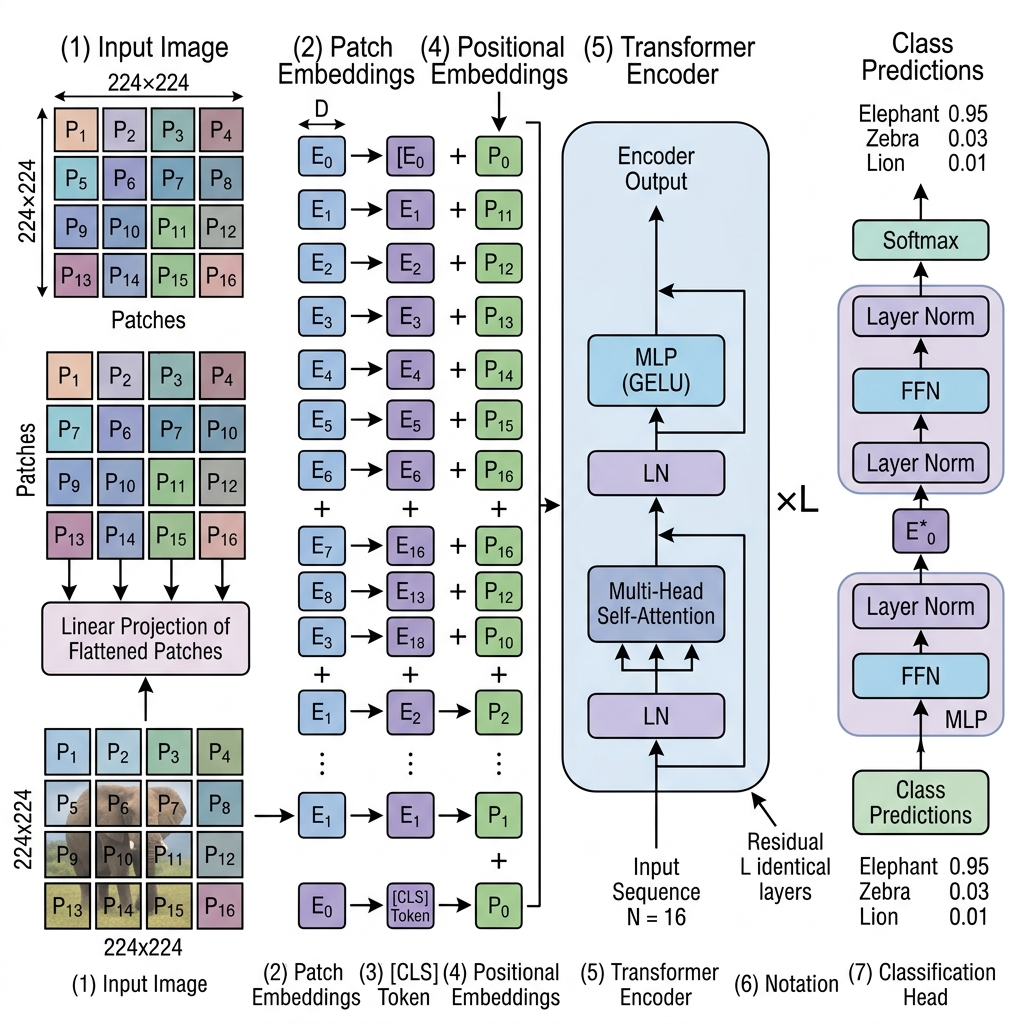
\includegraphics[width=0.9\textwidth]{docs/images/vit_architecture.png}
\end{figure}
\newpage
\subsection{Đầu phân loại và tinh chỉnh}
Sau $L$ khối Transformer, đầu ra của token $[\text{CLS}]$ đi qua một lớp MLP phân loại:
\begin{equation}
    \hat{y} = \text{softmax}(W_\text{cls} \cdot \text{LN}(\mathbf{z}_L^0) + b_\text{cls})
\end{equation}
Mô hình được tiền huấn luyện trên ImageNet-21k (14 triệu ảnh, 21,843 lớp) rồi tinh chỉnh (fine-tune) trên tập dữ liệu lá lúa \texttt{prithivMLmods/Rice-Leaf-Disease} với 4 lớp đầu ra.

\begin{table}[H]{So sánh thông số của các biến thể ViT}
\centering
\begin{tabular}{lcccc}
\toprule
\textbf{Biến thể} & \textbf{Layers (L)} & \textbf{Hidden size (D)} & \textbf{Heads (h)} & \textbf{Params} \\
\midrule
ViT-Tiny  & 12 & 192  & 3  & 5.7M \\
ViT-Small & 12 & 384  & 6  & 22M \\
ViT-Base  & 12 & 768  & 12 & 86M \\
ViT-Large & 24 & 1024 & 16 & 307M \\
ViT-Huge  & 32 & 1280 & 16 & 632M \\
\bottomrule
\end{tabular}
\end{table}

\section{Mô hình ngôn ngữ lớn (LLM) và Gemini}

\subsection{Kiến trúc Transformer Decoder}
Trong khi ViT (Vision Transformer) sử dụng kiến trúc Transformer Encoder — nơi mỗi token có thể chú ý đến toàn bộ các token khác trong chuỗi theo cả hai chiều — các mô hình ngôn ngữ lớn thế hệ mới như GPT (OpenAI) hay Gemini (Google DeepMind) lại áp dụng kiến trúc Transformer Decoder với cơ chế causal self-attention (hay còn gọi là masked self-attention). Trong cơ chế này, mỗi token chỉ được phép chú ý đến chính nó và các token đứng trước đó trong chuỗi, hoàn toàn không có quyền truy cập vào các token phía sau. Thiết kế này đảm bảo tính nhân quả trong quá trình sinh văn bản: mô hình không thể "nhìn trước" tương lai khi đang dự đoán hiện tại.\\
\indent Nhiệm vụ huấn luyện cốt lõi của các mô hình này là dự đoán token tiếp theo trong chuỗi (next-token prediction) — tức là, cho trước một đoạn văn bản, mô hình học cách ước tính token nào có xác suất xuất hiện cao nhất ở vị trí kế tiếp. Tuy đây là một mục tiêu huấn luyện đơn giản, nhưng khi được áp dụng lặp đi lặp lại trên một kho ngữ liệu khổng lồ lên đến hàng nghìn tỷ token văn bản — bao gồm sách, bài báo, trang web, mã nguồn và nhiều dạng nội dung khác — mô hình buộc phải ngầm học các quy luật ngữ pháp, cấu trúc lập luận, kiến thức thực tế và thậm chí cả khả năng suy luận nhiều bước. Đây chính là cơ chế mà qua đó các mô hình ngôn ngữ lớn hấp thụ tri thức một cách rộng rãi và sâu sắc từ thế giới văn bản.

\subsection{Mô hình Gemini của Google DeepMind}
Gemini được biết đến là một họ mô hình đa phương thức tiên tiến do Google DeepMind nghiên cứu và phát triển, sở hữu khả năng vượt trội trong việc tiếp nhận và xử lý đồng thời nhiều loại dữ liệu đầu vào khác nhau bao gồm văn bản, hình ảnh, âm thanh và video chỉ trong cùng một lời nhắc (prompt) [5]. Trong phạm vi triển khai của đề tài, hệ thống đã lựa chọn sử dụng phiên bản Gemini 2.5 Flash. Đây là phiên bản được tối ưu hóa để đạt được sự cân bằng lý tưởng giữa tốc độ xử lý và độ chính xác của dữ liệu đầu ra, hoàn toàn phù hợp với các bài toán thực tế yêu cầu phản hồi trong một khoảng thời gian chờ đợi chấp nhận được.

Lý do chính yếu cho việc ưu tiên lựa chọn Gemini 2.5 Flash thay vì các phiên bản có cấu trúc phức tạp và mạnh mẽ hơn như Gemini Pro nằm ở vấn đề độ trễ (latency). Các kết quả thực nghiệm thực tế cho thấy, phiên bản Flash có khả năng trả về kết quả nhanh chóng trong khoảng $\approx$ 5–8 giây; trong khi đó, phiên bản Pro có thể kéo dài thời gian phản hồi lên tới 15–20 giây—một mức độ trễ được đánh giá là quá lâu và không đáp ứng được yêu cầu về trải nghiệm người dùng thực tế. Bên cạnh đó, tham số nhiệt độ sinh văn bản ($T$) cũng được thiết lập chuyên biệt cho từng tác vụ: mức $T$ được đặt ở 0.2 đối với Morphology Agent nhằm đảm bảo các mô tả hình thái mang tính khách quan và chính xác, trong khi mức $T$ được nâng lên 0.4 đối với Coordinator Agent để tạo ra các báo cáo có sự linh hoạt và uyển chuyển hơn về mặt ngôn ngữ.

Tuy nhiên, hệ thống vẫn tồn tại một số hạn chế nhất định cần được lưu ý như việc sử dụng Gemini API bắt buộc phải có kết nối Internet ổn định và bị ràng buộc bởi giới hạn số lượng lượt gọi theo định mức của gói miễn phí. Hiện tại, hệ thống vẫn chưa có cơ chế tự động xử lý trong các tình huống API bị quá tải hoặc xảy ra gián đoạn kết nối—đây được xác định là những điểm trọng yếu cần được nghiên cứu và cải thiện trong các phiên bản nâng cấp tiếp theo.

\section{RAG và ChromaDB}

\subsection{Vấn đề Hallucination của LLM}
Mặc dù các mô hình ngôn ngữ lớn (LLM) hiện nay sở hữu khả năng xử lý và tạo lập ngôn ngữ vô cùng phi thường, chúng vẫn tồn tại một hạn chế cố hữu là xu hướng xảy ra hiện tượng "ảo giác" (hallucination). Đây là trạng thái mà mô hình tự bịa đặt ra những thông tin nghe có vẻ rất hợp lý và thuyết phục về mặt ngôn từ, nhưng về bản chất lại hoàn toàn sai lệch so với thực tế. Trong bối cảnh chuyên biệt như ngành nông nghiệp, những sai sót này không chỉ dừng lại ở mức độ thông tin thuần túy; chẳng hạn, một khuyến nghị sai lệch về liều lượng sử dụng thuốc bảo vệ thực vật có thể trực tiếp dẫn đến những thiệt hại nghiêm trọng về kinh tế và cây trồng. 
\newpage Để giải quyết vấn đề này, RAG (Retrieval-Augmented Generation) được ứng dụng như một giải pháp chủ chốt nhằm kiểm soát và giảm thiểu hiện tượng "ảo giác". Bằng cách truy xuất và cung cấp các ngữ cảnh thực tế từ một kho tri thức đã được kiểm chứng và xác thực độ tin cậy, RAG buộc mô hình phải dựa trên các căn cứ xác thực thay vì tự suy diễn, từ đó đảm bảo tính chính xác cho các phản hồi đầu ra.

\subsection{Kiến trúc RAG}
RAG bổ sung một bước truy xuất thông tin vào quy trình sinh văn bản, gồm hai giai đoạn:

\textbf{Giai đoạn Lập chỉ mục (Indexing --- offline):}
\begin{enumerate}[leftmargin=1.5cm]
    \item \textbf{Nạp tài liệu:} Các tài liệu về bệnh học cây lúa, phác đồ điều trị.
    \item \textbf{Phân đoạn (Chunking):} Chia tài liệu thành các đoạn (chunk) nhỏ.
    \item \textbf{Nhúng (Embedding):} Chuyển đổi mỗi chunk thành vector số học chiều cao bằng mô hình embedding.
    \item \textbf{Lưu trữ:} Lưu các vector vào cơ sở dữ liệu vector (ChromaDB).
\end{enumerate}

\textbf{Giai đoạn Truy vấn (Query --- online):}
\begin{enumerate}[leftmargin=1.5cm]
    \item Câu hỏi người dùng được nhúng thành vector bằng cùng mô hình embedding.
    \item Tìm kiếm tương đồng vector trong ChromaDB để lấy $k$ tài liệu liên quan nhất.
    \item Ghép tài liệu truy xuất + câu hỏi gốc thành một lời nhắc (prompt) cho LLM.
    \item LLM sinh câu trả lời dựa trên ngữ cảnh thực tế được cung cấp.
\end{enumerate}

\begin{figure}[H]{Kiến trúc pipeline RAG hai giai đoạn: Indexing (lập chỉ mục offline) và Query (truy vấn online). ChromaDB đóng vai trò là kho lưu trữ vector trung tâm.}
    \centering
    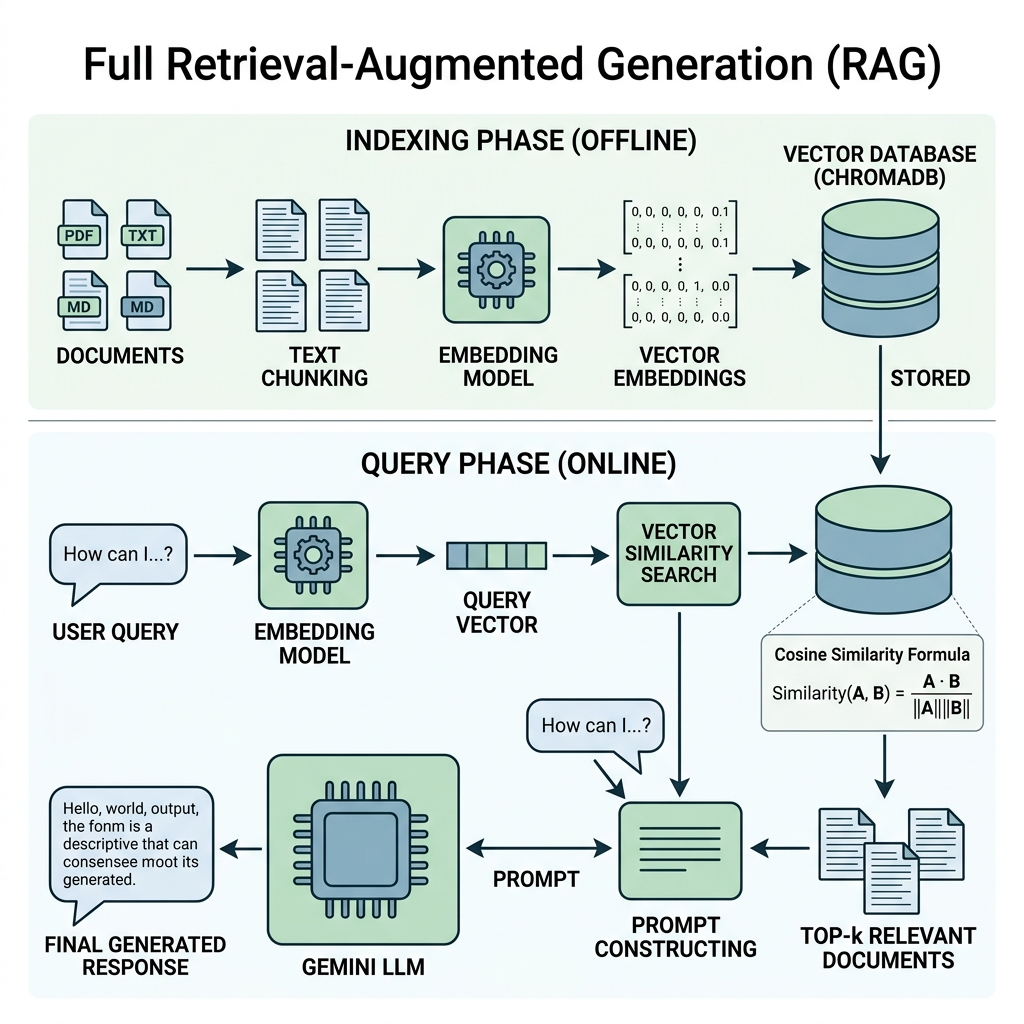
\includegraphics[width=0.8\textwidth]{docs/images/rag_pipeline.png}
\end{figure}

\subsection{Độ tương đồng Cosine}
Phép đo quan trọng nhất trong tìm kiếm vector là độ tương đồng cosine --- đo góc giữa hai vector thay vì khoảng cách Euclidean, do đó không bị ảnh hưởng bởi độ dài vector:
\begin{equation}
    \text{sim}(\mathbf{A}, \mathbf{B}) = \cos(\theta) = \frac{\mathbf{A} \cdot \mathbf{B}}{\|\mathbf{A}\|\|\mathbf{B}\|} = \frac{\displaystyle\sum_{i=1}^{n} A_i B_i}{\sqrt{\displaystyle\sum_{i=1}^{n}A_i^2} \cdot \sqrt{\displaystyle\sum_{i=1}^{n}B_i^2}}
    \label{eq:cosine}
\end{equation}
Giá trị $\text{sim} \in [-1, 1]$; trong không gian embedding thực tế, $\text{sim} \in [0, 1]$. Hệ thống chỉ truy xuất tài liệu với $\text{sim} > 0.82$ để đảm bảo độ liên quan.

\subsection{ChromaDB}
ChromaDB đóng vai trò là cơ sở dữ liệu vector mã nguồn mở (phát hành dưới giấy phép Apache 2.0), được thiết kế với kiến trúc tối ưu chuyên biệt cho các tác vụ của quy trình Thế năng tăng cường truy xuất (RAG). Một trong những đặc điểm nổi bật nhất của ChromaDB là khả năng lưu trữ cục bộ trực tiếp trên ổ đĩa (persistent storage), giúp dữ liệu được duy trì bền vững mà không nhất thiết phải thiết lập hay quản lý một hệ thống server riêng biệt, từ đó đơn giản hóa cấu hình hệ thống. Trong quá trình triển khai, ChromaDB thể hiện khả năng tương thích cao thông qua việc tích hợp trực tiếp với khung làm việc LangChain thông qua thư viện langchain-community, giúp quá trình kết nối và điều phối dữ liệu trở nên liền mạch.

Về mặt chức năng, hệ thống hỗ trợ cơ chế lọc theo siêu dữ liệu (metadata filtering), cho phép người dùng thực hiện các truy vấn tinh lọc dựa trên các tiêu chí cụ thể như loại bệnh lý hoặc nguồn tài liệu nguồn, giúp thu hẹp phạm vi tìm kiếm và tăng độ chính xác của thông tin truy xuất. Để đảm bảo hiệu suất vận hành, ChromaDB sử dụng thuật toán chỉ mục HNSW (Hierarchical Navigable Small World). Đây là một thuật toán tiên tiến cho phép thực hiện các phép tìm kiếm láng giềng gần đúng (Approximate Nearest Neighbor) một cách cực kỳ hiệu quả, duy trì tốc độ phản hồi nhanh ngay cả khi phải xử lý trên các tập dữ liệu có quy mô lớn.

\section{Lý thuyết AI Agent}

\subsection{Định nghĩa AI Agent}

AI Agent (Tác nhân trí tuệ nhân tạo) là một hệ thống có khả năng hoạt động một cách tự chủ để hoàn thành các nhiệm vụ được giao, thông qua việc thiết kế các workflow (luồng công việc) sử dụng các công cụ có sẵn \cite{ibm2025}. Một AI Agent thường không chỉ thực hiện xử lý ngôn ngữ tự nhiên (NLP), mà còn có khả năng ra quyết định, giải quyết vấn đề, tương tác với môi trường bên ngoài và thực hiện các hành động liên quan để đạt được mục tiêu.

Tại lõi của AI Agent thường là một mô hình ngôn ngữ lớn (LLM). Những mô hình này được sử dụng để hiểu yêu cầu của người dùng, tạo ra các bước xử lý và quyết định thời điểm gọi đến các công cụ bên ngoài (tool calling) khi cần thiết. Trong nhiều tài liệu, AI Agent còn được gọi là ``LLM agents'' do vai trò trung tâm của LLM trong kiến trúc của nó \cite{sumers2023}.

Cần phân biệt AI Agent với các khái niệm liên quan: một \textbf{AI Assistant} (trợ lý AI) phản hồi trực tiếp theo từng yêu cầu của người dùng và dừng lại khi hoàn thành câu trả lời, trong khi AI Agent có khả năng tự lập kế hoạch, tự đặt ra các nhiệm vụ phụ và tiếp tục hành động mà không cần giám sát liên tục từ con người. Ranh giới quan trọng nhất là \textbf{tính tự chủ}: Agent có thể quyết định \emph{khi nào} và \emph{bằng công cụ nào} để hoàn thành mục tiêu, còn Assistant chỉ đưa ra kết quả theo yêu cầu tức thời.

\subsection{Các đặc điểm nổi bật của AI Agent}

Năm đặc điểm chính phân biệt AI Agent với các hệ thống AI truyền thống \cite{sumers2023}:

\textbf{Tự chủ (Autonomy):} AI Agent có khả năng đưa ra quyết định mà không cần sự can thiệp liên tục từ người dùng trong từng bước. Nó có thể tự tạo các nhiệm vụ phụ (subtasks) để hoàn thiện mục tiêu tổng thể. Đây là đặc điểm cốt lõi nhất phân biệt Agent với một hàm xử lý thông thường.

\textbf{Kết hợp công cụ bên ngoài (Tool-calling):} Khi nội tại của mô hình không đủ kiến thức hoặc khả năng, AI Agent có thể gọi các API, truy vấn cơ sở dữ liệu, sử dụng các mô-đun chuyên biệt hoặc thậm chí tương tác với các Agent khác để thu thập thông tin hoặc thực hiện tác vụ. Nhờ vậy, nó có thể cập nhật thông tin thời gian thực, xử lý dữ liệu mới và mở rộng khả năng giải quyết các nhiệm vụ phức tạp. Trong hệ thống của đề tài, mỗi Agent chính là một ``công cụ'' mà Coordinator Agent gọi đến theo trình tự.

\textbf{Bộ nhớ và khả năng học từ tương tác (Memory \& Reflection):} AI Agent có khả năng lưu giữ thông tin từ các tương tác trước --- tức là có ``nhớ'' --- để tinh chỉnh cách hoạt động, phản hồi và đáp ứng theo sở thích người dùng. Nó học từ phản hồi của người dùng hoặc từ các Agent khác, sử dụng dữ liệu đó để tự điều chỉnh và cải thiện dần theo thời gian. Trong hệ thống hiện tại, bộ nhớ được thể hiện thông qua ChromaDB lưu trữ tri thức bệnh học bền vững qua các phiên làm việc.

\textbf{Khả năng lập kế hoạch \& lý luận (Planning \& Reasoning):} AI Agent phân tích mục tiêu cấp cao, phân rã thành các bước con, đưa ra kế hoạch hành động để đạt mục tiêu. Trong quá trình thực thi, nó cũng thực hiện reasoning (lý luận) để đánh giá lại kế hoạch, tự hiệu chỉnh và chọn phương án tối ưu dựa trên thông tin mới thu thập được. Coordinator Agent trong đề tài thực hiện vai trò này bằng cách quyết định thứ tự gọi các Agent phụ và cách tổng hợp kết quả cuối cùng.

\textbf{Khả năng thích ứng và mở rộng (Adaptivity \& Scalability):} Nhờ học hỏi và phản hồi liên tục, AI Agent có thể thích ứng với đặc điểm riêng của người dùng hoặc ngữ cảnh cụ thể. Khi được triển khai trong kiến trúc đa tác nhân (multi-agent), nó có thể phối hợp với các Agent khác để mở rộng khả năng, tăng hiệu quả và tính linh hoạt. Kiến trúc của đề tài được thiết kế để thêm một Agent mới chỉ cần viết một lớp Python và đăng ký vào Coordinator, không cần thay đổi các Agent hiện có.

\subsection{Phân loại AI Agent}

Dựa trên mức độ phức tạp và khả năng ra quyết định, AI Agent được phân thành năm loại chính từ đơn giản đến phức tạp \cite{sumers2023}:

\textbf{Simple Reflex Agent (Tác nhân phản xạ đơn giản):} Là dạng kiến trúc cơ bản nhất, hoạt động hoàn toàn dựa trên sự phản ứng trực tiếp với trạng thái hiện tại của môi trường theo các quy tắc điều kiện--hành động được định sẵn. Tác nhân chỉ xem xét những gì nó cảm nhận được ngay tại thời điểm hiện tại để ra quyết định, bỏ qua kinh nghiệm trong quá khứ cũng như không tính đến hệ quả tương lai. Ưu điểm là tốc độ và độ đơn giản; hạn chế là không xử lý được môi trường thay đổi hoặc tình huống ngoại lệ.

\textbf{Model-Based Reflex Agent (Tác nhân phản xạ dựa trên mô hình):} Phiên bản nâng cao tích hợp thêm một mô hình nội tại về thế giới (world model), cho phép lưu trữ và theo dõi trạng thái môi trường qua thời gian, hiểu được cách các hành động trong quá khứ đã ảnh hưởng đến trạng thái hiện tại. Nhờ đó, tác nhân có thể ra quyết định chính xác hơn ngay cả khi không thể quan sát đầy đủ môi trường tức thời.

\textbf{Goal-Based Agent (Tác nhân dựa trên mục tiêu):} Không chỉ phản ứng với trạng thái hiện tại mà còn lập kế hoạch hành động hướng đến một mục tiêu cụ thể. Tác nhân đánh giá nhiều chuỗi hành động khác nhau và chọn chuỗi dẫn đến trạng thái mong muốn, thường sử dụng các thuật toán tìm kiếm và lập kế hoạch. Đây là nền tảng lý thuyết cho Coordinator Agent trong đề tài: mục tiêu là báo cáo chẩn đoán hoàn chỉnh, kế hoạch là gọi 4 Agent phụ theo đúng thứ tự.

\textbf{Utility-Based Agent (Tác nhân dựa trên độ hữu dụng):} Mở rộng từ Goal-Based bằng cách không chỉ tìm kiếm trạng thái mục tiêu mà còn tối ưu hóa chất lượng của kết quả đạt được thông qua hàm độ hữu dụng (utility function). Khi có nhiều cách đạt mục tiêu, tác nhân chọn phương án tối ưu nhất theo tiêu chí đã xác định (ví dụ: nhanh nhất, ít tốn kém nhất, độ chính xác cao nhất).

\textbf{Learning Agent (Tác nhân học):} Đây là loại Agent tiên tiến nhất, có thể cải thiện hiệu năng theo thời gian thông qua kinh nghiệm tích lũy. Learning Agent gồm bốn thành phần: (1) phần tử học (learning element) để cải thiện từ phản hồi, (2) phần tử thực thi (performance element) để đưa ra hành động, (3) phần tử phê bình (critic) để đánh giá kết quả, và (4) phần tử tạo vấn đề (problem generator) để khám phá trạng thái mới. Đây là hướng phát triển tương lai cho hệ thống: nếu có cơ chế thu thập phản hồi từ nông dân, hệ thống có thể học và tinh chỉnh dần theo thời gian.

\subsection{So sánh AI Agent và AI Assistant}

Một điểm dễ gây nhầm lẫn là sự khác biệt giữa AI Agent và AI Assistant. Bảng~\ref{tab:agent_vs_assistant} tóm tắt các khác biệt chính:

\begin{table}[H]{So sánh AI Agent và AI Assistant}
\label{tab:agent_vs_assistant}
\centering
\begin{tabularx}{\textwidth}{>{\bfseries}p{3.2cm} X X}
\toprule
\textbf{Tiêu chí} & \textbf{AI Assistant} & \textbf{AI Agent} \\
\midrule
Tính tự chủ & Thấp --- phản hồi theo yêu cầu tức thời & Cao --- tự lập kế hoạch và hành động \\[4pt]
Trí nhớ & Ngắn hạn, trong cửa sổ ngữ cảnh & Bền vững, lưu trữ qua các phiên \\[4pt]
Phạm vi công cụ & Hạn chế theo API được lập trình sẵn & Kết nối sâu với hệ thống bên ngoài \\[4pt]
Vai trò hành động & Đề xuất, con người quyết định & Tự thực hiện hành động đầu cuối \\[4pt]
Phân rã nhiệm vụ & Không tự phân rã & Tự tạo subtask để đạt mục tiêu \\[4pt]
Phối hợp & Độc lập & Phối hợp với Agent khác trong hệ sinh thái \\
\bottomrule
\end{tabularx}
\end{table}

Phản hồi của AI Assistant là kết quả trực tiếp của yêu cầu hiện tại, không có khả năng tiếp tục hành động khi được hướng dẫn thêm. Trong khi đó, AI Agent thể hiện tính tự chủ cao hơn. Sau khi nhận mục tiêu ban đầu, chúng có thể tự phân tích, suy luận, lập kế hoạch và hành động mà không cần sự giám sát liên tục của con người. AI Agent còn có thể tự đặt ra nhiệm vụ phụ, điều chỉnh chiến lược khi điều kiện thay đổi và hoàn thành mục tiêu theo cách tối ưu nhất \cite{ibm2025}.

Trong đề tài này, hệ thống được thiết kế theo mô hình \textbf{Goal-Based Multi-Agent}: mỗi Agent phụ (Preprocessing, Classification, Morphology, Retrieval) hoạt động như một Simple Reflex Agent chuyên biệt, còn Coordinator Agent đóng vai trò Goal-Based Agent điều phối toàn bộ quy trình hướng đến mục tiêu là báo cáo chẩn đoán cuối cùng.

\subsection{Hệ thống Đa Tác Nhân (Multi-Agent System)}

Một Hệ thống Đa Tác Nhân (MAS --- Multi-Agent System) là tập hợp nhiều Agent tự trị cùng hoạt động và phối hợp trong một môi trường chung để giải quyết các bài toán phức tạp mà một Agent đơn lẻ không thể xử lý hiệu quả. Mỗi Agent trong hệ thống có thể có mục tiêu riêng, nhưng hành động của chúng được điều phối để đạt được mục tiêu chung của toàn hệ thống.

Ưu điểm của kiến trúc MAS so với một Agent đơn hoặc pipeline đơn thuần:

\begin{itemize}[leftmargin=1.5cm]
    \item \textbf{Phân chia trách nhiệm (Separation of Concerns):} Mỗi Agent chuyên trách một nhiệm vụ cụ thể, giúp code dễ bảo trì và kiểm thử độc lập.
    \item \textbf{Khả năng mở rộng:} Thêm năng lực mới vào hệ thống chỉ cần thêm Agent mới mà không cần thay đổi các Agent hiện có.
    \item \textbf{Chịu lỗi tốt hơn (Fault Tolerance):} Nếu một Agent gặp lỗi, Coordinator có thể xử lý ngoại lệ mà không làm sập toàn bộ hệ thống.
    \item \textbf{Phối hợp tự trị:} Các Agent có thể phối hợp theo luồng điều phối (orchestration) hoặc tự thương lượng (negotiation) tùy theo kiến trúc.
\end{itemize}

\subsection{Mô hình phối hợp trong hệ thống}
Hệ thống sử dụng mô hình phối hợp \textbf{Orchestrated Sequential}: Coordinator Agent đóng vai trò nhạc trưởng, điều phối luồng thực thi tuần tự (preprocessing $\rightarrow$ classification $\rightarrow$ morphology $\rightarrow$ retrieval $\rightarrow$ report). Mô hình này được chọn thay vì song song hoàn toàn vì mỗi bước phụ thuộc vào đầu ra của bước trước: Classification Agent cần ảnh đã tiền xử lý; Morphology Agent cần biết nhãn bệnh để định hướng phân tích; Coordinator Agent cần đủ bốn kết quả để tổng hợp.

Một điểm thiết kế quan trọng là cơ chế \textbf{callback theo dõi tiến trình}: thay vì đợi toàn bộ pipeline chạy xong rồi trả kết quả, Coordinator gọi hàm \texttt{progress\_callback(msg)} sau mỗi bước. Giao diện Streamlit lắng nghe callback này và cập nhật thẻ trạng thái Agent ngay lập tức, tạo cảm giác đáp ứng nhanh dù tổng thời gian xử lý vẫn có thể mất $\sim$15 giây.

So sánh với phương án pipeline đơn giản (hàm gọi hàm theo thứ tự cứng), kiến trúc Agent mang lại hai lợi thế thực tế: (1) dễ thay thế từng Agent mà không ảnh hưởng các Agent khác --- ví dụ thay Gemini bằng một LLM khác chỉ cần sửa file \texttt{morphology.py}; (2) dễ kiểm thử độc lập từng Agent bằng unit test mà không cần chạy cả hệ thống.